% 编译（在 0913 目录）：先编译 trajectory_dataflow_20260929.tex，再对本文件运行两次 xelatex。
% 报告内容以 2026-09-29 本次重构的工作区及已有验证产物为依据。
\documentclass[UTF8,fontset=fandol,a4paper,10pt]{ctexart}
\usepackage[margin=19mm,headheight=14pt]{geometry}
\usepackage{amsmath,amssymb,booktabs,tabularx,array,longtable,graphicx,pdflscape}
\usepackage{xcolor,enumitem,fancyhdr,listings,xurl,hyperref}
\definecolor{ink}{HTML}{203B51}
\definecolor{teal}{HTML}{087F8C}
\hypersetup{colorlinks=true,linkcolor=teal,urlcolor=teal,pdftitle={轨迹生成与统一接口重构报告},pdfauthor={项目技术报告}}
\pagestyle{fancy}\fancyhf{}\lhead{轨迹生成与统一接口重构报告}\rhead{2026-09-29}\cfoot{\thepage}
\setlength{\parindent}{2em}\setlength{\parskip}{4pt}
\setlist[itemize]{leftmargin=1.5em,itemsep=3pt,topsep=3pt}
\renewcommand{\arraystretch}{1.3}
\newcolumntype{Y}{>{\raggedright\arraybackslash}X}
\newcommand{\code}[1]{{\small\nolinkurl{#1}}}
\newcommand{\file}[1]{{\small\path{#1}}}
\newcommand{\note}[1]{\par\noindent\colorbox{teal!8}{\parbox{\dimexpr\linewidth-2\fboxsep\relax}{#1}}\par}
\lstset{basicstyle=\ttfamily\footnotesize,breaklines=true,columns=fullflexible,keepspaces=true,frame=single,rulecolor=\color{ink!25}}
\begin{document}
\begin{center}
{\LARGE\bfseries 轨迹生成与统一接口重构报告}\\[5pt]
{\large 三类解析轨迹、自定义八字与当前数据传输架构}\\[4pt]
{\small 2026-09-29 \quad 仓库：many\_controllerV3 \quad 对象：本次未提交工作区改动}
\end{center}
\section{本次改动与结论}
本次按 \file{0913/}轨迹生成/\file{uav_trajectory_design.tex} 重建水平加速圆、竖直俯仰翻转圆、水平轴滚转螺旋，并以自定义水平八字替换 \code{set_2D8_ref()}。保留 omtraj 优化器及其离线 CSV 路径，删除其余旧轨迹生成器。轨迹层现在直接输出统一运动参考，三个外环控制器共享同一输入契约。

\note{本次重点是\textbf{重构轨迹源并完成接口收口}。\code{ReferenceWindow} 和下层角加速度前馈消息在此前已经存在，本次没有新创一套 ROS 消息协议；实际变化是去除旧轨迹适配链，分离模式信息，并保留解析轨迹的高阶导数直至控制器。}

\par\noindent\begin{tabularx}{\linewidth}{@{}p{24mm}YY@{}}\toprule
项目 & 重构前 & 本次结果\\\midrule
轨迹实现 & minimum-snap、barrel-roll、five-turn、旧八字等多条实现路径 & 一个连续时间解析核心覆盖三类主体轨迹及八字；omtraj 独立保留\\
八字入口 & \code{set_2D8_ref()} 及旧八字生成器 & \code{figure_eight}，与其他轨迹共用参数选择、播放器和窗口接口\\
轨迹传输 & 旧轨迹结果和适配层参与参考转换 & 解析源直接返回 \code{ReferencePoint}；仅 CSV 边界转换 omtraj 结果\\
模式与运动 & 旧参考结构承担多种职责 & 运动走 \code{ReferenceWindow}；模式走 \code{ControlModeReference}，不重复传输 $p,v,a$\\
时间与前馈 & 离散缓存及差分路径限制轨迹表达 & 按真实时刻求未来点；解析源提供 jerk、snap、角速度与角加速度\\
终端行为 & 旧五圈参考首尾存在残余角速度 & 新解析轨迹以 $C^4$ 连接进入显式静止悬停\\
参数选择 & 存在 CMD 轨迹编译宏及控制器专用路径 & 启动读取 \code{trajectory.type}；三个控制器使用同一轨迹入口\\\bottomrule
\end{tabularx}\par

\subsection{相较旧方案，合理性体现在哪里}
几何尺寸与时间律可以直接解释：主体圆直径不超过 2 m，螺旋主体每圈推进 0.5 m；高阶运动量来自同一条连续曲线，连接和终端有明确的连续性约束；用项目实际质量、惯量与电机分配参数进行逐电机名义检查，而非只检查总推力。接口不再要求新轨迹伪装成旧优化器结果。

默认竖直圆和螺旋的名义峰值推力加速度约为 $2.8g$，低于此前旧五圈样例的约 $6.67g$。但圈数、时间律和推进量不同，\textbf{这不能等价为同一任务下闭环跟踪性能已提升}。本次已完成构建、31 项单元测试和名义采样检查，尚无完整闭环仿真或实飞结论。

\clearpage
\section{新轨迹如何生成}
\subsection{空间曲线与时间律分离}
以下为主体曲线，省略统一平移量 $p_0$；$r$ 为半径，$h$ 为每圈轴向推进量，$L,W$ 为八字全长、全宽。起飞、稳定和连接段另行拼接。
\begin{align*}
p_{\rm horizontal}(\theta)&=(r(\cos\theta-1),\ r\sin\theta,\ 0)^\top,\\
p_{\rm vertical}(\theta)&=(r\sin\theta,\ 0,\ r(1-\cos\theta))^\top,\\
p_{\rm helix}(\theta)&=(h\theta/(2\pi),\ r\sin\theta,\ r(1-\cos\theta))^\top,\\
p_{8}(\theta)&=((L/2)\sin\theta,\ (W/2)\sin2\theta,\ 0)^\top.
\end{align*}
水平圆和八字使用七阶速度包络及其积分：
\[
 H(u)=35u^4-84u^5+70u^6-20u^7,\qquad
 G(u)=7u^5-14u^6+10u^7-\tfrac52u^8.
\]
加速段为 $\dot\theta=\Omega H(t/T_r)$，减速段对称。水平圆的 \code{turns} 表示匀速阶段圈数，加减速还会贡献相位，因此结束点不强制回到主体起点；八字的 \code{turns} 表示包含加减速的总圈数，自动调整匀速时长使总相位闭合。八字采用 $\Omega=v_{\max}/\sqrt{(L/2)^2+W^2}$ 限制速度上界。

竖直圆与螺旋主体保持 $\dot\theta=\sqrt{A/r}$、$A=1.8g>g$，以保留圆顶正推力余量。直径从设计文档候选的 4 m 收缩至 2 m 后，在同一向心加速度下角速度增大 $\sqrt{2}$ 倍，故检查覆盖重新设计后的整段动作。

\subsection{连接、姿态与终端}
起飞与连接段采用归一化时间九次多项式，匹配两端 $p,v,a,j,s$，保证位置 $C^4$；这属于边界插值，不能称为最小 snap 优化。螺旋用独立轴向加减速段建立、消除前进速度，避免与滚转连接同时发生导致偏航分配峰值。

以 $a+g e_3$ 恢复推力方向，通过辅助轴投影构造姿态：竖直圆使用辅助 $y$ 轴，其他使用辅助 $x$ 轴。由 jerk、snap 解析求 $\omega,\alpha$，保留倒飞分支并拒绝奇异构型。四元数符号锚点仅选择 $q$ 或 $-q$，不参与运动量插值。新解析轨迹终点及之后满足 $v=a=j=s=\omega=\alpha=0$、$a_T=g$。

\subsection{当前默认参数}
\par\noindent\begin{tabularx}{\linewidth}{@{}p{29mm}Y@{}}\toprule
类型 / 公共项 & 默认参数\\\midrule
公共起飞 & 相对 CMD 激活位置上升 1.5 m，3 s；稳定 0.5 s\\
水平加速圆 & 半径 1 m，匀速 2 圈，速度 1.5 m/s；加、减速各 3 s\\
竖直翻转圆 & 半径 1 m，1 圈，$A=1.8g$；进出各 0.85 s、1.43 m\\
水平轴螺旋 & 半径 1 m，2 圈，推进 0.5 m/圈，$A=1.8g$；独立轴向过渡各 1 s\\
翻转公共连接 & 悬停点比圆底高 1.1 m；主体相对激活位置高度约 0.4--2.4 m\\
水平八字（默认） & 全长 2 m，全宽 1.2 m，总计 2 圈；速度上限 1.5 m/s，加减速各 3 s\\\bottomrule
\end{tabularx}\par
\note{\textbf{尺寸边界：}代码要求 $0<r\leq1$ m，约束的是主体圆。默认翻转进出连接使相应水平方向总跨度约 2.86 m；螺旋进出段另有轴向位移。完整动作并不被限制在 2 m 立方体内。}

\clearpage
\section{统一接口与数据契约}
\subsection{上层运动参考}
\code{Trajectory::evaluate(t)} 返回单个 \code{ReferencePoint}。\code{TrajectoryPlayer} 负责激活时间、起点位置和航向对齐，每个控制周期生成：
\[
 t_k=t_{\rm now}-t_0+k\Delta t,\quad k=0,\ldots,H;\qquad
 \mathcal W=\{\text{stamp},\Delta t,\mathrm{ReferencePoint}_{0:H}\}.
\]
新解析轨迹精确求值这些时刻，不进行旧缓存插值。播放器拒绝时钟回退。悬停、降落等非 CMD 参考也经外推与姿态解算形成同一窗口；手动模式允许空运动窗口。

\par\noindent\begin{tabularx}{\linewidth}{@{}p{44mm}YY@{}}\toprule
字段 / 结构 & 含义与单位 & 约定\\\midrule
\code{position/velocity/acceleration} & $p,v,a$；m、m/s、m/s$^2$ & 局部世界系，$z$ 向上\\
\code{jerk/snap} & $j,s$；m/s$^3$、m/s$^4$ & 解析源来自同一曲线\\
\code{attitude} & 单位四元数 & 参考机体系到世界系\\
\code{thrust_acceleration} & $a_T=T/m$；m/s$^2$ & 不是 N，也不是油门\\
\code{body_rate/body_acceleration} & $\omega,\alpha$；rad/s、rad/s$^2$ & 参考机体系 FLU\\
\code{full_state} & 完整姿态/推力/角速度是否为权威值 & 区别平坦输出待解析与完整参考\\
\code{kinematics_valid} & $p$ 至 snap 是否来自同一可微曲线 & 新解析源为真，CSV 不虚构导数\\
\code{angular_acceleration_valid} & 角加速度是否有意义 & 有效零与缺失值必须区分\\
\code{ControlModeReference} & 模式、手动态度、油门、航向速率及有效标志 & 独立于运动窗口，不含重复 $p,v,a$\\\bottomrule
\end{tabularx}\par
内部世界系必须与反馈一致：当前 PX4 桥使用 NED 到 NWU 的转换 $[x,y,z]\mapsto[x,-y,-z]$，不能直接当作标准 ENU。轨迹对齐时世界系向量旋转和平移，机体系 $\omega,\alpha$ 不重复旋转。

\subsection{控制器与下层消息}
三个控制器公共入口统一为运动窗口与模式信息。当前编译选择 \code{PX4CTRL_PRIMARY_CONTROLLER=2}：acados NMPC；0 为 QuadControl，1 为 OmMPC。外环 100 Hz，内环 400 Hz。NMPC 默认 $H=12,\Delta t=0.04$ s，即 13 点、0.48 s；OmMPC 默认 9 点、0.08 s；QuadControl 使用单点。\textbf{外环周期不等于预测网格间隔。}

外环输出 \code{Control_Setpoint_t}，再发布 \code{/rates_thrust_setpoint}。\code{RatesThrustSetpoint} 消息沿用既有布局：微秒时间戳、总推力 N、机体角速度 rad/s、角加速度前馈 rad/s$^2$ 及其有效标志。位置轨迹、参考姿态和轨迹力矩不直接装入该消息。
\[
 \alpha_{\rm ff}^{B}=R_{\rm actual}^{\top}R_{\rm ref}\alpha_{\rm ref},\quad
 \alpha_{\rm cmd}=\mathrm{PID}(\omega_{\rm cmd}-\omega)+\alpha_{\rm ff}^{B},\quad
 \tau=I\alpha_{\rm cmd}+\omega\times I\omega.
\]
内环负责力矩计算、电机分配和油门映射，发布 \code{/fmu/in/actuator_motors}。轨迹静态检查得到的力矩只用于可行性审计，避免与内环重复叠加。

\clearpage
\begin{landscape}\thispagestyle{empty}
\section{当前数据传输架构图}
\begin{center}
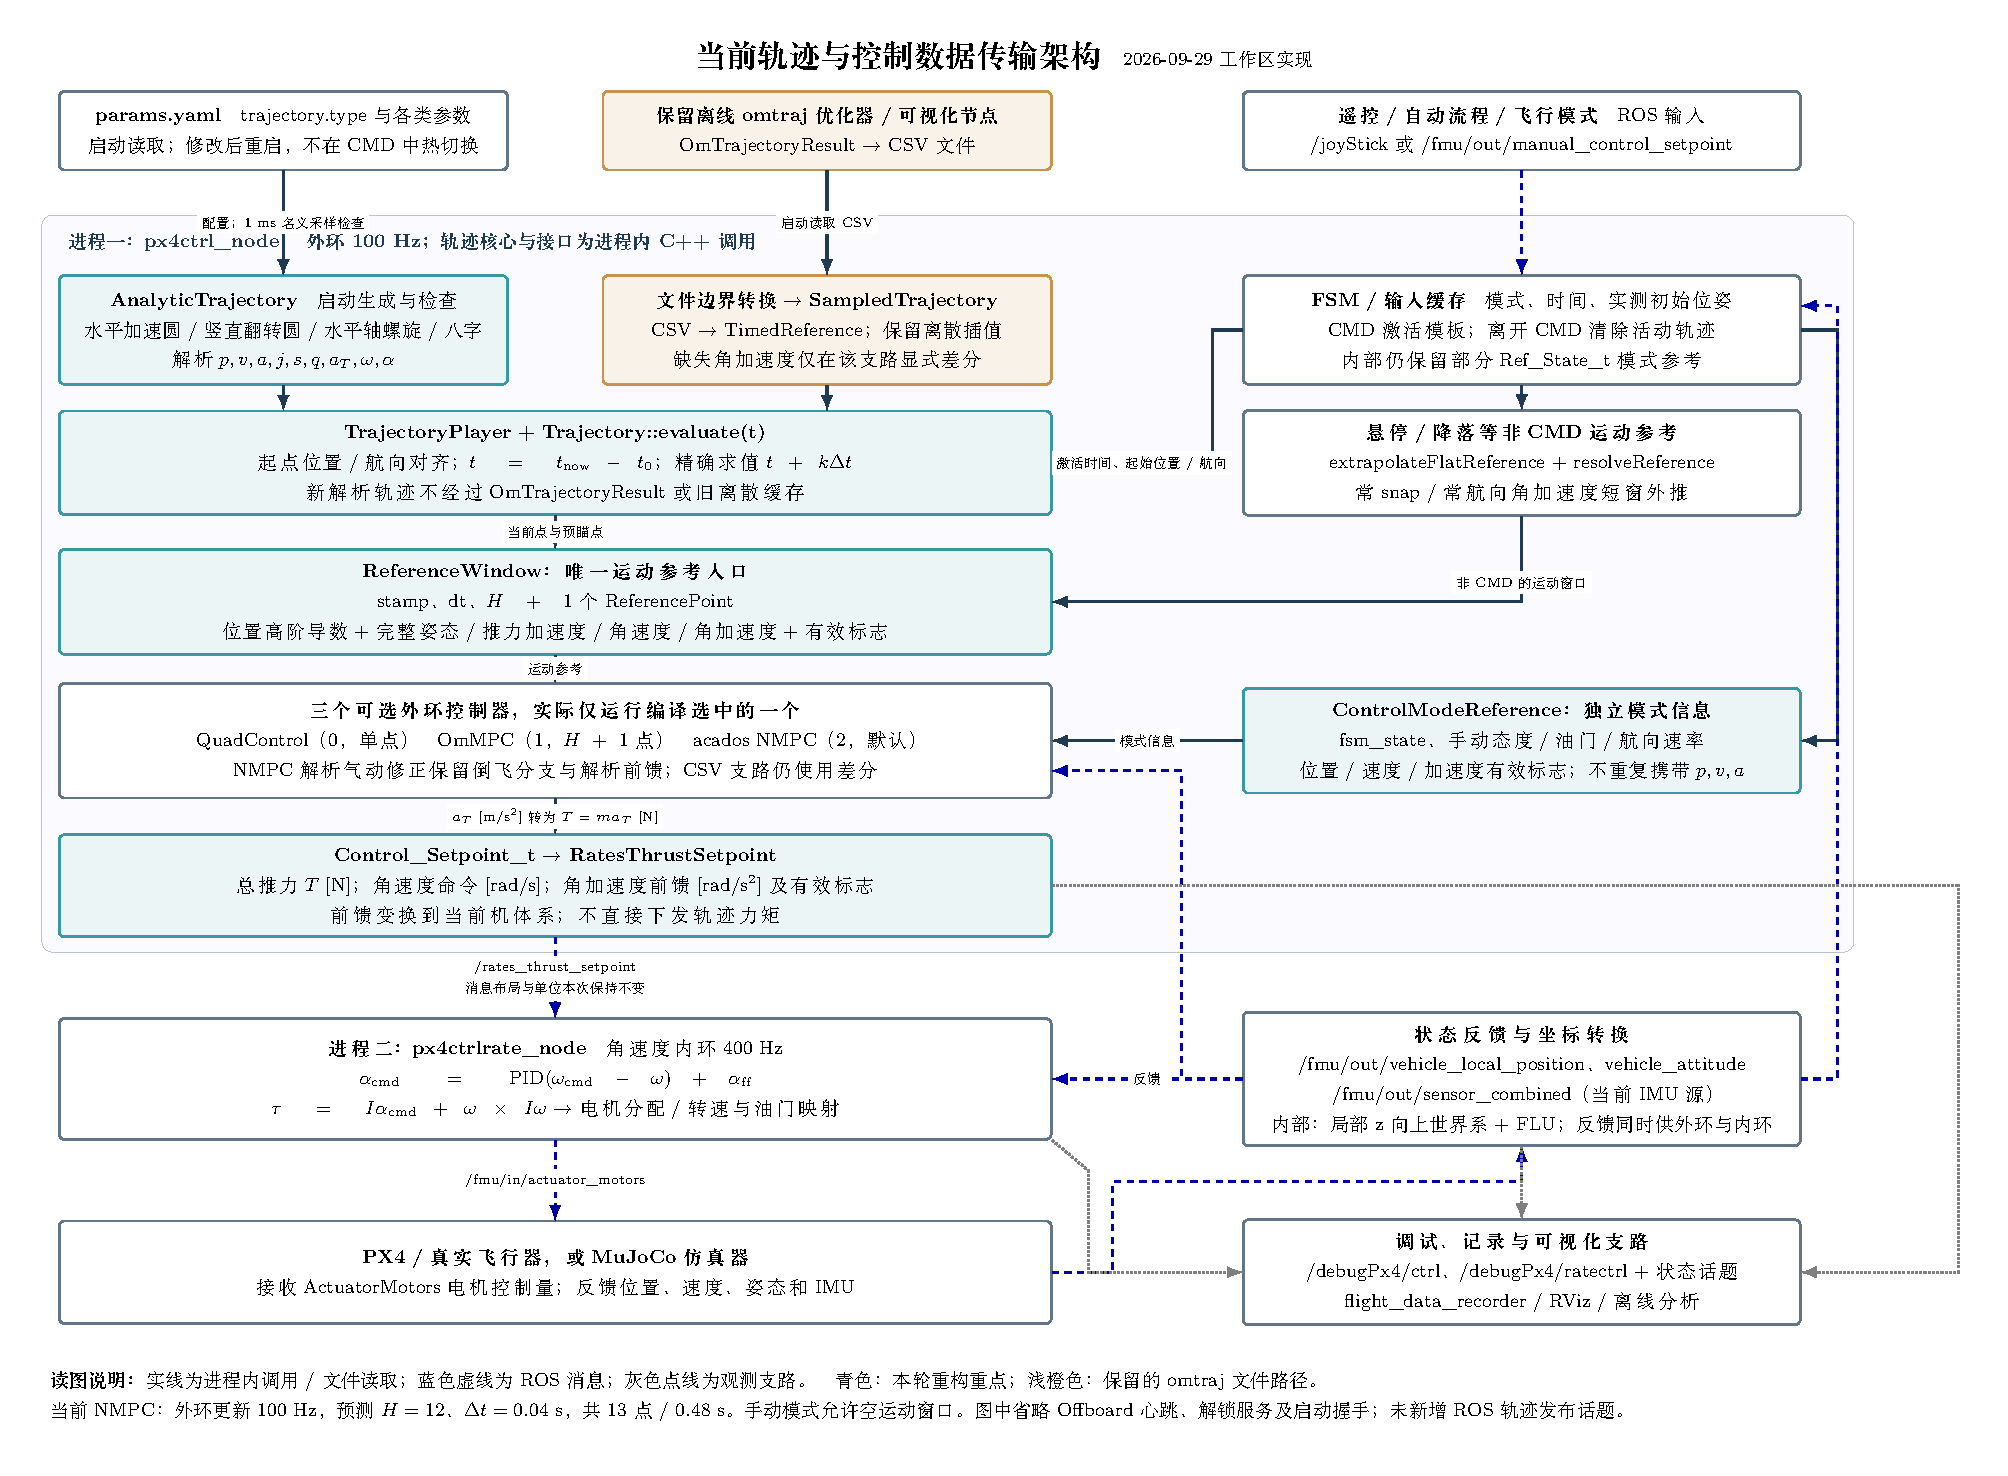
\includegraphics[width=\linewidth,height=.85\textheight,keepaspectratio]{trajectory_dataflow_20260929.pdf}
\end{center}
\noindent\small 图中参考窗口和下层消息承接此前接口工作；青色标出本次重点改动区域。轨迹与播放器位于外环进程内，没有新增独立 ROS 轨迹节点。可编辑图源为 \file{trajectory_dataflow_20260929.tikz.tex}，独立图文档为 \file{trajectory_dataflow_20260929.tex}。
\end{landscape}

\clearpage
\section{代码修改清单与运行行为}
下表路径除特别注明外，均相对 \file{src/realflight_modules/px4ctrl/}；成对的头文件、源文件分别位于 \code{include/px4ctrl/} 与 \code{src/}。
\par\noindent\begin{tabularx}{\linewidth}{@{}p{13mm}p{58mm}Y@{}}\toprule
类别 & 文件 / 模块 & 作用\\\midrule
新增 & \code{trajectory.h/.cpp} & 通用轨迹接口、四类解析轨迹、播放器、名义约束检查\\
新增 & \code{sampled_trajectory.h/.cpp} & 通用离散轨迹、插值、缺失角加速度重建与终端 HOLD\\
新增 & \code{omtraj_reference.cpp} & CSV 在源边界转为 \code{TimedReference}，隔离优化器结果类型\\
新增 & \code{trajectory_inspect.cpp} & 无 ROS 副作用的检查、CSV 导出工具\\
新增 & \code{test/trajectory_test.cpp} & 10 项轨迹及跨接口回归测试\\
新增 & \file{script/analyze_trajectories.py} & 读取实际 YAML，导出冻结参数、指标、四条 CSV 与曲线图（仓库根目录下）\\
修改 & \code{control_reference.h/.cpp} & 模式结构分离、运动学有效标志、倒飞几何解算、解析气动导数\\
修改 & \code{controller}、\code{ommpc}、\code{acados_nmpc} & 统一控制器公共入口；解析源气动补偿保持解析角加速度\\
修改 & \code{px4ctrlfsm.h/.cpp}、\code{px4ctrl_node.cpp} & 启动准备轨迹、CMD 激活与清理、运行时参数选择；移除旧八字专用入口\\
修改 & \code{CMakeLists.txt}、\code{config/params.yaml} & 库边界调整，新增工具/测试与统一轨迹参数\\
删除 & \code{minimum_snap_trajectory}、\code{barrel_roll_trajectory}、\code{five_turn_trajectory}、\code{figure_eight_trajectory}、\code{legacy_trajectory_reference} & 删除上述五组头/源文件；移除 \code{set_2D8_ref()} 与 \code{PX4CTRL_CMD_TRAJECTORY}\\
文档 & \code{TRAJECTORIES.md}、\code{CONTROL_REFERENCE.md}；根目录项目说明与闭环分析说明 & 记录接口、参数与验证边界；旧分析时间窗需随新轨迹调整\\\bottomrule
\end{tabularx}\par

\subsection{保留与兼容范围}
omtraj 优化算法、离线可视化和 CSV 格式保留；新增转换器只在文件入口工作。omtraj 仍采用离散插值，从世界角速度差分补充缺失角加速度，不声称具有解析 jerk/snap。\code{Ref_State_t} 仍存在于 FSM 内部模式参考及 QuadControl 私有旧控制律中，但已经不是传递新轨迹的控制器公共接口。

本轮没有修改内环控制律、电机映射、\code{RatesThrustSetpoint} 消息定义或 acados 生成模型。气动补偿使用名义姿态进行一次修正并解析传播导数，不是气动力与姿态耦合方程的全局求解。

\subsection{启动、执行与异常处理}
启动按 YAML 的 \code{trajectory.type} 生成或加载轨迹，并执行参数和名义约束检查；失败拒绝启动对应控制流程。进入 CMD 时绑定实测位置、航向和时间，离开 CMD 时清除活动轨迹。配置更新需重启节点，目前不支持活动轨迹热切换。

入口假设激活时近似悬停，不根据任意实测非零速度重新规划。时钟回退或无效参考沿用 FSM 既有处理；本次未增加特技中断恢复规划器。

\clearpage
\section{量化结果与旧方案对比}
\subsection{当前默认参数的名义检查}
数据取自 \file{datalog/trajectory_refactor/metrics.json}。按 1 ms 采样\textbf{完整动作}，包括起飞、稳定、进出段和主体；使用实际 YAML 质量、惯量与分配参数。以下是无气动名义参考与静态电机分配结果，不是闭环实测数据。

\par\noindent\begin{tabularx}{\linewidth}{@{}Yrrrrr@{}}\toprule
轨迹 & 总时长 & 最大速度 & 最大 $a_T$ & 最大 $\|\omega\|$ & 最大 $\|\alpha\|$\\
 & s & m/s & m/s$^2$ & rad/s & rad/s$^2$\\\midrule
水平加速圆 & 17.878 & 1.500 & 11.367 & 0.443 & 1.139\\
竖直翻转圆 & 6.696 & 4.218 & 27.454 & 9.452 & 81.528\\
水平轴螺旋 & 10.191 & 4.231 & 27.454 & 9.452 & 81.528\\
水平八字 & 19.586 & 1.500 & 11.367 & 0.448 & 1.330\\\bottomrule
\end{tabularx}\par

\par\noindent\begin{tabularx}{\linewidth}{@{}Yrrc@{}}\toprule
轨迹 & 最小单电机推力 / N & 最大单电机推力 / N & 采样检查\\\midrule
水平加速圆 & 1.671 & 2.305 & 通过\\
竖直翻转圆 & 0.719 & 5.595 & 通过\\
水平轴螺旋 & 0.820 & 5.588 & 通过\\
水平八字 & 1.671 & 2.305 & 通过\\\bottomrule
\end{tabularx}\par

当前约束包括：逐电机推力不超过静态最大值的 70\%，角加速度模长不超过 100 rad/s$^2$，以及总推力、各轴角速度和相对高度检查。最低相对高度阈值为 $-0.01$ m；本次四条默认动作采样最小相对高度均为 0 m（起始点）。高度为相对激活点高度，不构成地形避障。

电机检查结合 $\tau=I\alpha+\omega\times I\omega$ 与当前内环实际电机编号解分配，能够发现总推力不高但某个电机超限的情况。默认模型质量为 0.811 kg，惯量为 $(1.91,2.37,3.60)\times10^{-3}$ kg\,m$^2$；采用项目现用动力参数，未照搬设计文档的候选电机参数。

\subsection{旧五圈样例的可比与不可比部分}
此前旧五圈 QP 样例为 15 s、约五圈，测得最大速度 7.65 m/s、最大推力加速度 65.42 m/s$^2$、最大角速度 10.85 rad/s，首尾残余角速度约 0.146 rad/s。新默认翻转类最大推力加速度约 27.45 m/s$^2$，并通过完整连接使解析终端角速度、角加速度归零。

这组数字支持“\textbf{当前默认动作更温和、端点定义更完整}”的判断。由于旧五圈与新默认的一圈竖直圆、两圈螺旋不是同一任务，不能直接据此给出控制精度或能耗提升比例。若要判断闭环优劣，需要固定几何、圈数和完成时间，再比较跟踪误差、求解失败、电机饱和与控制延迟。

\subsection{检查结果的适用边界}
\begin{itemize}
\item 1 ms 采样不是连续时间峰值的数学证明，也未覆盖电机动态、来流变化、电池限流和所有模型误差。
\item 默认连接参数已筛选检查，不意味着任意用户参数组合都会自动优化为可飞轨迹。
\item omtraj 的终点后返回 HOLD，但 CSV 最后一个非悬停输入到 HOLD 不保证 $C^4$；平滑终端仍需在离线优化任务中约束。
\end{itemize}

\clearpage
\begingroup\setlength{\parskip}{2pt}\renewcommand{\arraystretch}{1.12}
\section{验证记录、复现与后续验证项}
\subsection{本次重构已有验证记录}
本报告核对了上一阶段构建日志、测试 XML 和分析产物；编写报告时未因纯文档修改重复执行飞行控制构建。
\par\noindent\begin{tabularx}{\linewidth}{@{}p{48mm}p{23mm}Y@{}}\toprule
验证项 & 结果 & 主要覆盖内容\\\midrule
\texttt{colcon build}：px4ctrl & 通过 & 默认控制器下编译与链接\\
\code{trajectory_test} & 10 / 10 & 解析导数、$C^4$ 连接、终端悬停、倒飞、推进量、窗口时刻、非法参数、CSV 转换\\
\code{control_reference_test} & 6 / 6 & 统一参考解算与参考契约\\
\code{controller_adapter_test} & 2 / 2 & 控制器适配入口\\
\code{acados_nmpc_test} & 13 / 13 & 求解器路径、有效前馈及异常/手动清理等\\
控制器 0 / 1 编译路径 & 语法检查通过 & FSM 与 node 翻译单元；不等于两套完整链接或闭环验证\\
四类轨迹名义分析 & 全部通过 & 实际 YAML、1 ms 采样、静态逐电机预算\\\bottomrule
\end{tabularx}\par

4 个测试套件合计 \textbf{31 项通过}，XML 位于 \file{build/px4ctrl/test_results/px4ctrl/}。轨迹测试还覆盖气动修正后解析导数、倒飞参考进入 acados、跨圈四元数符号连续性，以及真实预测网格和刚体对齐。\texttt{git diff --check} 已通过。

\subsection{使用与复现}
在 \file{src/realflight_modules/px4ctrl/config/params.yaml} 中设置 \code{trajectory.type} 为 \code{horizontal_circle}、\code{vertical_circle}、\code{helix}、\code{figure_eight} 或 \code{omtraj}，然后重启控制节点。默认值为 \code{figure_eight}。
\begin{lstlisting}
# 在仓库根目录执行
source /opt/ros/humble/setup.bash
source install/setup.bash
colcon build --packages-select px4ctrl --symlink-install --cmake-args -DBUILD_TESTING=ON
ctest --test-dir build/px4ctrl -R '^(trajectory_test|control_reference_test|controller_adapter_test|acados_nmpc_test)$' --output-on-failure
python3 script/analyze_trajectories.py
\end{lstlisting}
分析脚本读取项目 YAML，输出到 \file{datalog/trajectory_refactor/}：冻结参数、四条 CSV、\code{metrics.json} 和 \code{trajectories.png}。直接运行 \code{trajectory_inspect} 使用其 C++ 默认模型；涉及项目实际参数对比时应使用 Python 脚本。

\subsection{仍需完成的性能验证}
完整 MuJoCo 闭环与实飞尚未执行。下一阶段应验证三类控制器实际运行、完整动作跟踪、内外环时序、电机饱和及动态响应，并单独验证倒飞过程中的模式中断与恢复。旧闭环脚本中依赖旧轨迹的时间窗口需要重新配置。

\subsection{报告与图的文件}
报告源文件为 \file{0913/trajectory_refactor_report_20260929.tex}；架构图源文件为同目录 \file{trajectory_dataflow_20260929.tex} 和 \file{trajectory_dataflow_20260929.tikz.tex}。对应 PDF 已编译，架构图同时提供 PNG。重编译时先生成架构图 PDF，再对报告运行两次 XeLaTeX。此报告对应当前工作区，不表示这些改动已提交到 Git；仓库当前忽略 \code{0913} 目录，文件仍已写入指定位置。
\endgroup
\end{document}
